\Lecture{Jayalal Sarma}{August, 12 2015}{7}{Reduction of $\cal{GA}$ to $\cal{GI}$}{Sahil Sharma}

\newcommand{\cgi}{\mathcal{COLOR-GI}}
\newcommand{\compiso}{{\sf COMPUTE-ISO}}
\newcommand{\gi}{\mathcal{GI}}
\newcommand{\ga}{\mathcal{GA}}
\newcommand{\setstab}{ {\sf SETSTAB}}
\section{Recap and Lecture overview}
Let us denote by $\cgi$ the problem of finding whether there is a coloring
preserving isomorphism.  In the previous few lectures we showed that $\cgi \le
\gi$. We also showed that $\gi \le \ga$. We also showed how to compute an
isomorphism map between two graphs (\compiso) if we can check if two graphs are
isomorphic. Recall that $Aut(X)$ is the group of all automorphisms of a given
graph $X$ and $\ga$ is the problem of obtaining a generator for $Aut(X)$.  
In this lecture, we show that $\ga \le \gi$. That is, given a
subroutine to solve $\gi$, we show how we can compute a generator set of
$Aut(X)$ for an input graph $X$. Along with
$\gi \le \ga$ proved in the earlier class, this shows that the graph
isomorphism and graph automorphism problems are equivalent in terms of
hardness.

The main idea is that there is a unique way to express an element in
$G$ using Tower of subgroups of $G$.

\section{Solving Graph Automorphism using Graph Isomorphism}

\subsection{Tower of Subgroups of Group}
\begin{definition}[Tower of Subgroups of $G$]
	Let $k \in \N$. For a group $G$, the $k$ subgroups of $G$ namely
	$G^{(1)}, G^{(2)}, \ldots,  G^{(k)} = \{id\}$ is said to form a tower
	of subgroups of $G$ if \[ G = G^{(0)} \ge G^{(1)} \ge ,\ldots ,
	G^{(k)} = \{id\} \] 
\end{definition}
%The discussion in this section sets up the notation and concepts related to
%towers of subgroups of any given group $G$. 
The above concept is defined for an arbitrary group, but we will use this
specifically for understanding about Tower of subgroups of $Aut(X)$, for a
given graph $X$.

Note that in the sequence, $G^{(i)}$ is a subgroup of $G^{(i-1)}$ for $ 1 \le i
\le k$. Hence there is a coset structure that $G^{(i)}$ generates (or induces) 
in $G^{(i-1)}$ and we seek to exploit this structure to get a $O(n\log n)$
sized generating set of $Aut(X)$ efficiently, given a procedure for solving 
$\gi$. 
\begin{figure}[htp!]
	\centering
	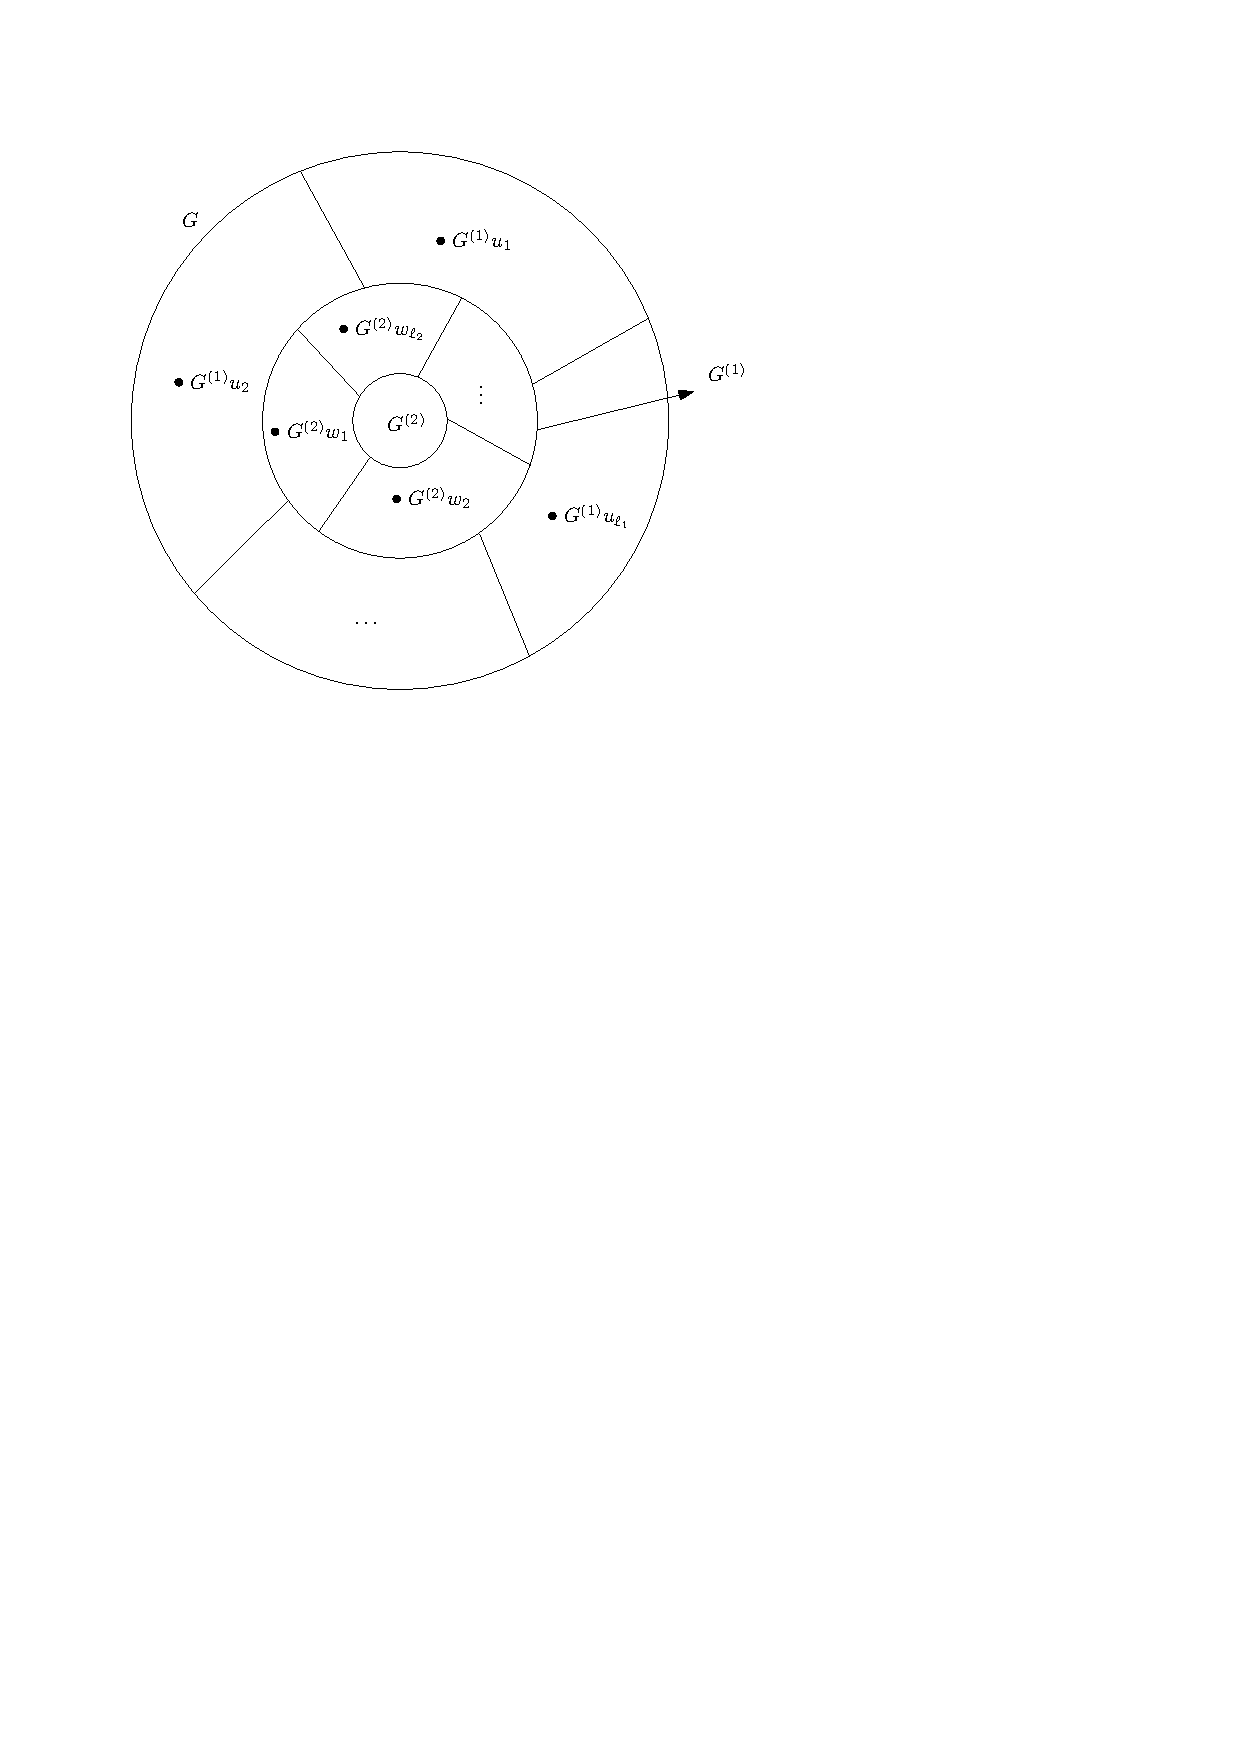
\includegraphics[scale=0.8]{images/tower}
	\caption{Tower of groups of $G$ for two levels with cosets in the
		first level fixed as $u_1,u_2,\ldots, u_{\ell_1}$ and second
		level fixed as $w_1,w_2,\ldots,w_{\ell_2}$.}
	\label{fig:tower}
\end{figure}

\begin{definition}
	For a group $G$ and a subgroup $H$ of $G$ denote $H:G$ to denote the
	set of cosets of $H$ in $G$ and the number of cosets in $H:G$,
	denoted, $[H:G]$ is called as the index of $H$ in $G$.
\end{definition}

For example, for $1\le i \le k$, $[G^{(i+1)}:G^{(i)}]$ denotes the number of
cosets of induced in $G^{(i)}$ by $G^{(i+1)}$. Denote this number by $\ell_i$.
Note that by Lagrange's theorem $\ell_i = \frac{|G^{(i)}|}{|G^{(i+1)}|}$.
Hence $\prod_{i} \ell_i = |G^{(0)}| = |G|$.

Recall the notion of a {\it coset representative} of a coset, with respect a
given group and a subgroup of the given group. For example, in the
figure~\ref{fig:tower}, consider the subgroup $G^{(1)}$ of $G$. Here we choose
$u_1$ as the coset representative of the coset $G^{(1)}u_1$.

Note that any arbitrarily chosen element of that coset $G^{(1)}u_1$ can be
made its representative due to the following reason. For any two elements in
the same coset, say $g$ and $g'$ we have $G^{(1)}g = G^{(1)}g'$, by the
definition of the coset (since it generates the same coset)\footnote{One way
	to show this is as follows : let $g, g' \in G^{(1)}u_1$ where $u_1$ is
	a coset representative. Hence $g = h_1u_1$, $g' = h_2u_2$ for $h_1,h_2
	\in G^{(1)}$. For any $w \in G^{(1)}g$, $w = hg$ for some 
	$h \in G^{(1)}$. Using the fact that $g = h_1u_1$, we get $w = hh_1u_1$.
	Hence $w \in G^{(1)}u_1$. Hence $G^{(1)}g \subseteq G^{(1)}u_1$. 
	A similar argument shows that $G^{(1)}u_1 \subseteq G^{(1)}g$. This
	also shows that $G^{(1)}u_1 = G^{(1)}g'$. Hence the cosets formed by
$g$ and $g'$ are the same as the original coset.}.  Hence, there is nothing
special about $u_1, g, g'$ and any elements of the coset can be chosen as its
representative.

\subsection{Unique representation of a group in terms of coset representatives}
Given this setup, we are now ready to give a unique way of representing group
elements once we fix a tower of subgroups for the group and a coset
representatives at each level.

Consider an element $g \in G^{(i-1)}$ for some $i \ge 1$ and $G^{(i+1)}$ be the
subgroup in the next level in the tower of subgroups. Since the cosets of
$G^{(i+1)}$ partitions $G^{(i)}$ it must be that $g$ must lie in exactly one
coset.

\begin{observation}
	Consider the groups $G^{(i)}$ and $G^{(i-1)}$ for some $i \ge 1$. 
	Let $g \in G^{(i-1)}$ lie in the coset whose representative is $u_1$.
	Then there exists a unique $h_i \in G^{(i)}$ such that \[ g = h_iu_1\]
	\label{obs:coset-rep-unique}
\end{observation}
\begin{proof}
	By definition, $g \in G^{(i)}u_1 \implies \exists h_{i} \in G^{(i)}$
	such that $g = h_{i}.u_{1}$. Such a $h_{i}$ is unique since if there
	is another $h_i' \in G^{(i)}$ such that $h_{i}u_1 = h_i'u_1$, then $
	h_i = g.u_{1}^{-1} = h_{i}'$.
\end{proof}
This gives us a way to uniqely represent the elements of $G$.
\begin{theorem}
	Suppose we fix the tower of subgroups of $G$ denoted 
	$G = G^{(0)} \ge G^{(1)} \ge , \ldots, G^{(k)} = \{id\}$ as well as 
	the coset representatives for $G^{(i+1)}:G^{(i)}$ for all $0 \le i \le
	k-1$ in the tower of subgroups. Then, each element of the group $G$
	can be represented as a unique product of coset representatives.
	\label{th:tower-coset-repr}
\end{theorem}
\begin{proof}
	Let $g \in G = G^{(0)}$. Let $\ell_1$ be the number of cosets in
	$G^{(1)}:G^{(0)}$. Let $u_1, u_2, \ldots, u_{\ell_1}$ be the coset
	representatives. By the above
	observation~\ref{obs:coset-rep-unique} (setting $i=1$), we know that 
	there exists a unique $h_{1} \in G^{(1)}$ such that $g = h_1u_1$. Now
	consider the cosets $G^{(2)}:G^{(1)}$. Since they partition $G^{(1)}$, 
	we ask, in which coset does $h_{1}$ belong to ? By the application of 
	the same claim to $h_{1}$ and the pair of groups
	$(G_{1}, G_{2})$ we get a unique $h_{2}$ such that $h_{1} =
	h_{2}u_{2}$, where $u_2$ is the coset in which $h_{1}$ belongs. Hence
	$g$ can be expressed as $h_2u_2u_1$.  
	
	Continuing in this way, as we go
	down the tower of subgroups while fixing the coset representations, 
	in each stage we get a unique $h_i$ and $u_i$ whose product gives
	$h_{i-1}$ and we end up with a unique representation for the element
	$g$. Note that this representation is unique since at each stage the
	$h_{i}$ were found in a unique way, and the coset-representatives are
	fixed.
\end{proof}
Note that this also gives us a way to solve $\# \ga$. If we can count the
number of coset representatives at each level (which is $\ell_i$ by our
notation), then $\prod_i \ell_i = |G|$.

\subsection{Finding a generating set for $Aut(X)$}
To find a generating set for $Aut(X)$ it suffices to find a tower of
sub-groups of $Aut(X)$ and the coset representatives at each level.

Applying Theorem~\ref{th:tower-coset-repr} for $Aut(X)$, we can represent each
element of $Aut(X)$ uniquely as a product (which in our case is composition
operation) of a sequence of coset representatives once we define a
suitable tower of subgroups for $Aut(X)$ and compute the coset representatives
efficiently. Hence it suffices to output these representatives to obtain a
generating set.

We define the tower of subgroups in such a way that computing the coset
representatives becomes efficient (using $\cal{GI}$). Denote $G^{(0)}$ as
$Aut(X)$. The subgroups are defined as, for $0 \le i \le n-1$,
$$G^{(i+1)} := \{ g \in G^{(i)} ~|~ i^{g} = i\}$$
That is, $G^{(i)}$ is the sub-group of automorphisms which maps all the nodes
of the graph in the range $\{1, \ldots, i\}$ to themselves. 

We can check that $G^{(i)}$ is indeed a group since the composition of two
permutations which maps all the nodes of the graph in the range $\{1, \ldots,
i\}$ to themselves also does the same. Moreover, the
identity permutation is the identity for this sub-group too, and the inverse
permutation is defined in the standard way and satisfy the property of inverse
element of a group. 
% and has the same properties as the inverse permutation in $Aut(X)$. 
Hence, this is indeed a subgroup. By the definition of $G^{(i)}$ it can be
verified that the subgroups defined indeed forms a tower of subgroups of
$Aut(X)$.

Now the task is reduced to finding the coset representatives of $G^{(i+1)}$ in
$G^{(i)}$.  

\begin{claim}
Let the number of cosets generated by $G^{(i+1)}$ in $G^{(i)}$ be
$\ell_{i}$. Then $$\ell_{i} \le n-i$$
\end{claim}
\begin{proof}
Consider $g \in G^{(i)}$. Note that $g$ maps the element $i+1$ to an
element in the range $\{i+1, \ldots, n\}$. This is because the other elements
are already fixed. Let $k = (i+1)^{g}$ be the element to which $i+1$ is mapped
and $r$ be the element such that $r^{g}= i+1$. Then consider the permutation
$g'$ which retains other mappings from $g$ but changes the above two mappings
to $(i+1)^{g'} = i+1$ and $r^{g'} = k$. Note that $g'$ is also an automorphism
since $r$ being mapped to $i+1$ implies that if $r$ is mapped to the image of
$i$ the automorphism would still be preserved (adjacency and non-adjacency is
preserved). Also note that $g'$ maps $\{1, \ldots , i+1\}$ and hence is in
$G^{i+1}$. This means that whatever is the number of automorphisms in $G^{i}$
cannot exceed the number of automorphisms in $G^{i+1}$ multiplied by $n-i$
since the $i+1$ can potentially map to only $n-i$ elements.  
\end{proof}

This claims shows that at each level the number of representatives that we
need to output is at most $n-i$ and hence the size of generating set collected
over all levels is at most $\sum_{i=1}^n (n-i) = O(n^2)$.
The algorithm for finding the coset representatives is the following. We
explain how to get the representatives for a level $i$.

Look for automorphisms in $G^{(i)}$ which map all of $\{1, \ldots, i\}$ to
themselves and map $i+1$ to each element in the set $\{i+1, \ldots,n\}$, one
by one and ask the question: is there an automorphism which preserves these
mappings. This gives us the cosets since the only freedom in the coset
representatives is in where $(i+1)$ maps to. 

We answer this using $\cgi$ problem. Since we already have a solution to
$\gi$, as demonstrated in the previous lectures, we can use this to also 
solve $\cgi$. Now, this can done by using $\cgi$ in the following way. 

\begin{enumerate}
	\item Make two copies of the input graph $X$ and call it $X_1$ and
		$X_2$.
	\item Colour the vertex  $v_k \in \{v_1, \ldots, v_i\}$ by  with the
		color $k$ for both the graphs $X_1$ and $X_2$. 
	\item Colour the vertex $v_{i+1}$ in $X_1$ and $X_2$ with the same
		colour $i+1$ and use a new colour $i+2$ and colour the rest of 
		the vertices in both the graphs with the colour $i+2$.
\end{enumerate}

In this way, we can cast the problem as a $\cgi$ and solve it using
$\cal{GI}$. Each time we get an answer as yes, we then use the reduction
$\cgi \le \gi$ to find the actual permutation. This
permutation is one of the coset representatives and hence in this manner we
get each coset representative. Note that for each search for coset
representative we make only polynomially many calls to $\cal{GI}$ and the
number of such representatives is upper bounded by $n^2$ and hence our
reduction is polynomial time and computes a generating set of $Aut(X)$ in
polynomial time, given that we can solve $\cal{GI}$ in polynomial time.

Note that this procedure can me modified not only to compute an automorphism,
but can also be used to compute $|Aut(X)|$. The reason is that the $\ell_i$
which corresponds to number of coset representatives in $G^{(i+1)}:G^{(i)}$
can be exactly computed in our setting. Our final task is to obtain a
permutation in $G^{(i)}$ that sends $i+1$ to $\{i+1,\ldots,n\}$. The set of
permutations which satisfy this is nothing but the orbit of $i+1$ in
$G^{(i)}$. Hence by Orbit stabilizer theorem, $|G^{(i)}| = \left
|(i+1)^{G^{(i)}} \right |\ldots |G^{(i+1)}|$. This gives that $\left |
(i+1)^{G^{(i)}} \right | = \frac{|G^{(i)}}{|G^{(i+1)}|} = \ell_i$. This tells
that to obtain $\ell_i$ it suffices to estimate the size of the orbit of
$i+1$.

The generating set that we obtained by fixing a tower of subgroups and coset
representatives have many nice properties. We will see more about them in
subseqent lectures.
\begin{definition}[Strong Generating Set]
	A generating set for $Aut(X)$ obtained in the manner above making use
	of coset representatives and tower of sub-groups is known as a strong
	generating set.  
\end{definition}




\Lecture{Jayalal Sarma}{August, 14 2015}{8}{Some Group-theoretic
problems in Permutation Groups}{Sahil Sharma}
\section {Recap}
In the previous lecture we showed that $\cal{GA} \le \cal{GI}$. We also
defined certain generic group theoretic concepts like {\it tower of
sub-groups}, {\it coset representatives} and the notion of {\it strong
generating sets}.  Also note that the reduction $\cal{\#GA} \le \cal{GI}$ can
be done using the set of reductions ${\cal{\#GA} \le \cal{GA} \le \cal{GI}}$
where the first reduction follows from the fact that the generating set of
$Aut(X)$ was in fact a strong generating set and hence each element of $G$
could be obtained uniquely by composing elements of the generating set. 
This would imply that the size of the automorphism group is $\displaystyle
\prod_{i} \ell_{i}$ where $\ell_i$ is the number of cosets in the $i^{th}$
level of the tower of subgroups of $G$.

Our aim is to cast the graph theoretic problems in group theoretic terms and
solve the problem using the machinery of group theory.  Towards this aim, we
abstract the various problems and questions which were encountered while
doing the previous reductions and give a set of four related group-theoretic
problems.

\section{Some Computational Questions in Group theory}
Following are two natural question to ask.
\begin{problem}[Problem 1 (Order Computation)]
	Given a group $G$ via its generating set, can we compute the order of
	the group, that is, the number of elements in the group.
\end{problem}

%One of the things we will try to do to solve this problem is to convert the
%given generating set into a strong generating set. Since we already know how
%to solve the problem once that is done.

\begin{problem}[Problem 2 (Membership Testing)]
	Given an element  $g \in G$ and an $H \le G$ expressed via a
	generating set $S$ (i,e. $\langle S \rangle = H$), test if $g \in H$
	or not.
\end{problem}

Note that problem 2 can be solved using problem 1. This is because we could
just add $g$ to the generating set $S$ of $H$ and use problem $1$ to obtain
the sizes of the groups generated by $S$ and $S \cup \{g\}$. If the sizes are
unequal we conclude that $g$ was not in $H$. This is because if $g$ were in
$H$, then the generating set $S$ could have generated $g$ as well and adding
it to $S$ could not have resulted in any new elements.  

In last lecture, we also wanted to count the number of permutations in 
$G^{(i)}$ which first $i$ elements identically and maps the $i+1^{th}$ element
to any of the $n-i$ elements. We saw that this is actually a question of
obtaining the size of orbit. This motivates the following question.

\begin{problem}[Problem 3 (Orbit Computation)] 
	Given a group $G \le S_{n}$ (via its generating set $S$), compute the
	orbits of the action of $G$ on $[n]$.
\end{problem}

So far we were interested in groups which are subgroups of $S_n$. But how do
we answer the same questions for general abstract groups ? We show a different
way of viewing an abstract group can be looked at as a subgroup of a 
permutation group. 

\begin{claim}
	An group $G$ acts on itself. 
\end{claim}
\begin{proof}
Consider an element $g \in G$. Consider any arbitrary ordering of the elements
in $G$. Then the multiplication of $G$ by $g$, $G.g$ sends
the elements of $G$ to a permutation of themselves\footnote{The reason is that
	the resulting
operation acts bijectively on the elements. That is if $g_1 \ne g_2$ then
$gg_1 \ne gg_2$. Also for any $h = g_ix$, there is a unique solution $x =
hg_i^{-1}$ in $G$}. Hence, with each element
$g \in G$, we can associate a permutation of the elements of $G$ in the
following way : if $G = \{g_1,g_2,\ldots,g_k\}$. then for a $g_i \in G$,
corresponding $\sigma_i \in S_k$ is defined as the one which satisfy
$(g_ig_1,g_ig_2,\ldots,g_ig_n) = (g_{\sigma_i(1)}, g_{\sigma_i(2)}, \ldots, 
g_{\sigma_i(k)})$

Collect all the permutations associated with the group elements and call it
$H$. Note that the resulting set of permutations is forms a group since
multiplication in original group translates to composition in the new
group\footnote{ The statement amounts to showing that for 
	any $g_1,g_2 \in G$ with $\sigma_1, \sigma_2 \in H$ as
	the corresponding elements defined by the map, 
	$g_1g_2 \in G \iff \sigma_1 \circ \sigma_2 \in H$. This is because, 
	\begin{align*}
		g_1g_2 (g_1, g_2, \ldots, g_k) 
		= & (g_1 g_{\sigma_2(1)}, g_1 g_{\sigma_2(2)}, \ldots, 
		g_1 g_{\sigma_2(k)}) \\
		= & (g_{\sigma_1(\sigma_2(1))}, g_{\sigma_1(\sigma_2(2))},
		\ldots, g_{\sigma_1(\sigma_2(k))})
	\end{align*}
}
and the identity element in the original group is associated with the identity
permutation and so on.

Hence if the order of the group is $k$, then the resulting group of
permutations is a sub-group of $S_{k}$. This defines the notion of a group
acting on itself.
\end{proof}
\begin{note}
Hence from now on, we will assume that $G$ acts on an arbitrary set $\Omega$
which we can think $[n]$.
\end{note}

There is another motivation for studying this problem. We know, due to the 
orbit stabilizer lemma that for any $\alpha \in  G$, $$|\alpha^{G}|\cdot
|G_{\alpha}| = |G|$$ This gives us a recursive strategy to solve problem 1
(Order computation). Suppose we can estimate $|\alpha^{G}|$ which is the size
of the orbit, then to compute $|G|$, we are left with the smaller recursive
subproblem of estimating the size of $|G_{\alpha}|$. 

\section{Set Stabilizer Problem}
We know that $Aut(X)$ acts on $[n]$. This can also be visualized as $Aut(X)$
acting on the set of edges $E(X)$. This is because the automorphisms map edges
to edges and non-edges to non-edges. Hence, any edge of the graph gets maped
to another edge. Hence we can think of $Aut(X)$ as acting on the set of
edges.

Extending this idea, we can also think of $S_n$ which is a
super-group of $Aut(X)$ as acting on the set of all potential edges given by
$K = \{ \{i, j\} | i, j \in [n]$ and $i \le j\}$. Note that both these actions
are different in the following sense : permutations in $S_n$ need not map
edges to edges and non-edges to non-edges and hence edge set is not preserved
in the action, while permutations in $Aut(X)$ even
though maps different vertices differently, preserves the edge set. In other
words, the action of $Aut(X)$ on the set $E(X)$ does not changes $E(X)$ or it
\emph{fixes} $E(X)$. This leads us to the fourth problem called the \emph{Set
Stabilizer problem}

\begin{definition}[Set Stabilizer of $\Sigma$]
	Given a $G$ and a subset $\Sigma \subseteq \Omega$, 
	\[ 	\setstab(\Sigma) = \{ g \in G ~|~ \Sigma^{g} = \Sigma\} \]

	where $\Sigma^g = \{ \alpha^g ~|~ \alpha \in \Sigma \}$
\end{definition}

Given a group $G \le S_n$ which acts on a set $\Omega$, we define the Set
Stabilizer of $\Sigma \subseteq \Omega$ as the set of all permutations in $G$
which map elements of $\Sigma$ to elements of $\Sigma$ and all non elements of
$\Sigma$ to non-elements of $\Sigma$. Note that $\setstab(\Sigma)$ is a
sub-group of $G$. In the case of automorphism groups, the mapping is $G =
S_n$, $\Omega = K$, $\Sigma = E(X)$ and
$\setstab(\Sigma)$$=$$Aut(X)$.

Having set up all the notation, let us state the computational question we
seek to answer.
\begin{problem}[Problem 4 (Set Stabilizer Problem)]
Given a group $G$ via its generating set $S$, a set $\Omega$ on
which it acts and a subset $\Sigma \subseteq \Omega$, output a generating set
for the group $\setstab(\Sigma)$.
\end{problem}

By our previous discussion on $Aut(X)$ fixing the edges of $X$, we can
conclude that $Aut(X)$ is the stabilizer of $E(X)$. Hence the problem $\ga$
reduces to the problem $\setstab$.

\section{Solution to Problem 3 (Orbit Computation)}
For completeness's sake, let us restate the question. 

{\bf Orbit Computation} : Given a group $G \le S_{n}$ (via its generating set
$S$), compute the orbits of the action of $G$ on $[n]$.

We can see that the orbits of the action of $G$ on $[n]$ partition the set
into different subsets. Hence, we would want to compute the partitions. We
cast this problem as a graph theoretic problem.

Let $\Omega = [n]$. We construct a directed graph $X$ with $V(X) = \Omega$ and
$E(X) = \{(\alpha, \beta) ~ | ~ \exists g \in G, \beta = \alpha^g \} \subseteq
V(X) \times V(X)$.  We can have the edge $(\alpha, \beta) \in E(X)$ labelled
by $g \in G$ if $\alpha^g = \beta$. To check if two elements $\alpha, \beta$
lie in the same partition, it suffices to check if there is a directed path
from $\alpha$ to $\beta$ (or from $\beta$ to $\alpha$). Hence the connected
components of the graph corresponds to the orbits. In the next lecture, we
will give another algorithm for solving this problem.


%The vertices are the numbers in the set $[n]$.
%If $j \in [n]$ lies in the orbit of $i \in [n]$, then there is an edge from
%$i$ to $j$. We know due to the manner in which orbits are constructed and the
%fact that they induce partitions, the final graph looks like a set of
%cliques. Hence, we can try to compute the graph partitially (by finding some
%edges) and make use of transitive closures for finding the rest of the edges
%in the graph until we reach a fixed point, at which point we can say that we
%have computed the partition and hence the orbits.  
